\documentclass[xcolor=x11names,compress,professionalfonts]{beamer}

%% General packages %%%%%%%%%%%%%%%%%%%%%%%%%%%%%%%%%%
\usepackage[utf8]{inputenc}
\usepackage{graphicx}
\usepackage{tikz}
\tikzset{% change default arrow tips
    >=latex
}
\usepackage{ifthen}

\usepackage{amsmath}
\usepackage{nicefrac}

\usepackage{color}

%%%%%%%%%%%%%%%%%%%%%%%%%%%%%%%%%%%%%%%%%%%%%%%%%%%%%%


%% Beamer Layout %%%%%%%%%%%%%%%%%%%%%%%%%%%%%%%%%%
\useoutertheme[subsection=false,shadow]{miniframes}
\useinnertheme{rectangles}

\setbeamertemplate{navigation symbols}{}%remove navigation symbols

\usepackage{libertine}
\usepackage[T1]{fontenc}

\setbeamerfont{title like}{shape=\scshape}
\setbeamerfont{frametitle}{shape=\scshape}

\setbeamercolor*{lower separation line head}{bg=DeepSkyBlue4} 
\setbeamercolor*{normal text}{fg=black,bg=white} 
\setbeamercolor*{alerted text}{fg=red} 
\setbeamercolor*{example text}{fg=black} 
\setbeamercolor*{structure}{fg=black} 
 
\setbeamercolor*{palette tertiary}{fg=black,bg=black!10} 
\setbeamercolor*{palette quaternary}{fg=black,bg=black!10} 

\renewcommand{\(}{\begin{columns}}
\renewcommand{\)}{\end{columns}}
\newcommand{\<}[1]{\begin{column}{#1}}
\renewcommand{\>}{\end{column}}

\newcommand{\om}{\ensuremath{\omega}}
\newcommand{\lb}{\ensuremath{\overline{\lambda}}}
\newcommand{\zb}{\ensuremath{\overline{z}}}

\definecolor{BostonBlue}{HTML}{00688B}
\definecolor{Complementary}{HTML}{8B2300}
%%%%%%%%%%%%%%%%%%%%%%%%%%%%%%%%%%%%%%%%%%%%%%%%%%

\usepackage{braket}

%%%My Math

\newcommand{\pd}[2]{\frac{\displaystyle \partial #1}{\displaystyle\partial #2}} % for partial derivatives
\newcommand{\dx}{\mathrm{d}x}
\renewcommand{\d}[1]{\mathrm{d}#1}
\newcommand{\nth}{$n^\text{th}$ }

\newcommand{\mean}[1]{\langle #1 \rangle}
\DeclareMathOperator{\Pf}{Pf}
\DeclareMathOperator{\Tr}{Tr}

\begin{document}


\begin{frame}
\title{Electronic properties of quasicrystals}
%\subtitle{SUBTITLE}
\author{ Nicolas Macé, Anuradha Jagannathan, Frédéric Piéchon }
\date{
	June 24, 2015
}
\titlepage
\end{frame}

\section{Electronic properties of the Fibonacci chain.}
%Each section needs a subsection for the small points on top to show up
\subsection{Dummy}

\begin{frame}{Geometry of quasicrystals: the Fibonacci sequence}

\newcommand{\s}{.13}
  	\centering
    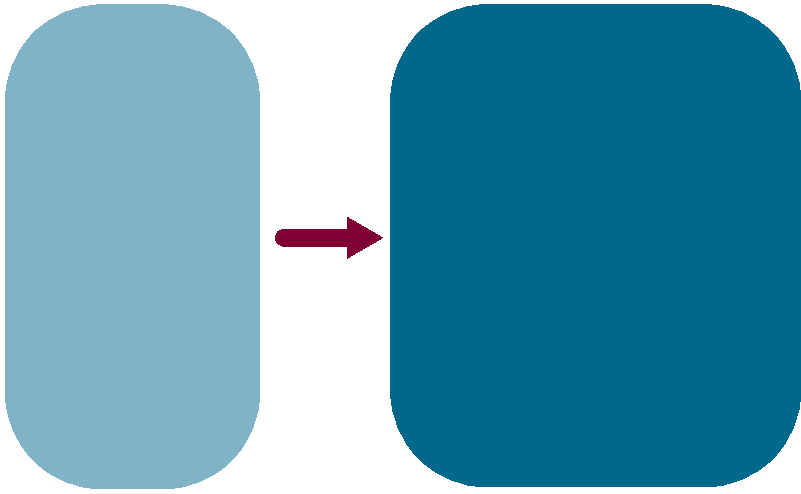
\includegraphics[scale=\s]{B_A.pdf}~~~~
    \includegraphics[scale=\s]{A_AB.pdf}
    
    ~\\
    \only<1>{\centering
    \includegraphics[scale=\s]{ABA.pdf}}
	\only<2>{\centering
    \includegraphics[scale=\s]{ABAAB.pdf}}
	\only<3>{\centering
    \includegraphics[scale=\s]{ABAABABA.pdf}}
    
\end{frame}

\begin{frame}{Geometry of quasicrystals: the Penrose tiling}

\newcommand{\s}{.35}
  	\centering
    \includegraphics[scale=\s]{dart_dart.pdf}~~~~
    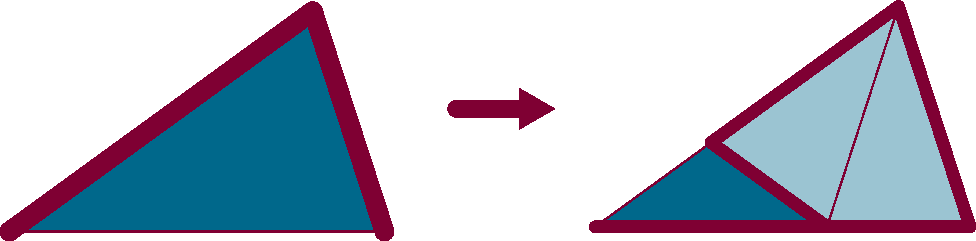
\includegraphics[scale=\s]{kate_kate.pdf}
    
    ~~~
    
    ~~\\
    \only<1>{\centering
    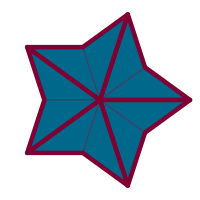
\includegraphics[scale=0.6]{Penrose_star_0.pdf}}
	\only<2>{\centering
    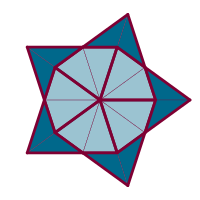
\includegraphics[scale=0.6]{Penrose_star_1.pdf}}
	\only<3>{\centering
    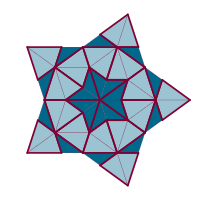
\includegraphics[scale=0.6]{Penrose_star_2.pdf}}
    
\end{frame}

\begin{frame}{Electron dynamics on quasiperiodic tilings}
    \begin{itemize}
    
    \item The Fibonacci sequence
    	\includegraphics[scale=0.12]{ABAABABA.pdf}
    
    \item The Fibonacci (tight binding) chain:
	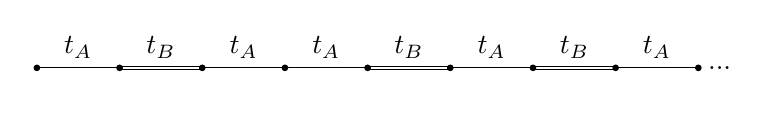
\begin{tikzpicture}[scale=.7]
    		\newcommand{\orig}{-1.5}
    		\newcommand{\trans}{1.5}
    		\newcommand{\vertspac}{-2.}
    	
    		% initial chain
    	
    		% bonds 
        	\draw[-] (\orig+\trans,0) -- (\orig+2*\trans,0) node [midway, above] {$t_A$};
			\draw[-,double] (\orig+2*\trans,0) -- (\orig+3*\trans,0) node [midway, above] {$t_B$};	
			\draw[-] (\orig+3*\trans,0) -- (\orig+4*\trans,0) node [midway, above] {$t_A$};
			\draw[-] (\orig+4*\trans,0) -- (\orig+5*\trans,0) node [midway, above] {$t_A$};
			\draw[-,double] (\orig+5*\trans,0) -- (\orig+6*\trans,0) node [midway, above] {$t_B$};
			\draw[-] (\orig+6*\trans,0) -- (\orig+7*\trans,0) node [midway, above] {$t_A$};
			\draw[-,double] (\orig+7*\trans,0) -- (\orig+8*\trans,0) node [midway, above] {$t_B$};
			\draw[-] (\orig+8*\trans,0) -- (\orig+9*\trans,0) node [midway, above] {$t_A$};
    	
    	
    		% sites
		    \filldraw (\orig+1*\trans,0) circle (0.05) node [below] {};
		    \filldraw (\orig+2*\trans,0) circle (0.05) node [below] {};
		    \filldraw (\orig+3*\trans,0) circle (0.05) node [below] {};
		    \filldraw (\orig+4*\trans,0) circle (0.05) node [below] {};
		    \filldraw (\orig+5*\trans,0) circle (0.05) node [below] {};
		    \filldraw (\orig+6*\trans,0) circle (0.05) node [below] {};
		    \filldraw (\orig+7*\trans,0) circle (0.05) node [below] {};
		    \filldraw (\orig+8*\trans,0) circle (0.05) node [right] {};
		    \filldraw (\orig+9*\trans,0) circle (0.05) node [right] {...};
		      
		\end{tikzpicture}
	\item Whenever $t_A \neq t_B$, the chain is quasiperiodic.
		\begin{itemize}
			\item Electron dynamics?
		\end{itemize}
	\end{itemize}
\end{frame}

\begin{frame}{Renormalization}

	\begin{itemize}
		\item Electron dynamics?
		\begin{itemize}
			\item No translational invariance: no Bloch theorem.
			\item But scale invariance: renormalization group approach!
		\end{itemize}
		
		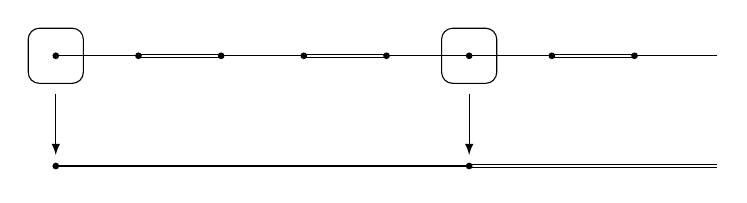
\begin{tikzpicture}[scale=.7]
    		\newcommand{\orig}{-1.5}
    		\newcommand{\trans}{1.5}
    		\newcommand{\vertspac}{-2.}
    		\newcommand{\vertsize}{.5} % vertical spand of the rectangles
    		\newcommand{\del}{.2}
    	
    		% initial chain
    	
    		% bonds 
        	\draw[-] (\orig, 0)  node [left] {}  -- (\orig+\trans, 0);
			\draw[-,double] (\orig+\trans,0) -- (\orig+2*\trans,0); % node [midway, above] {$t_s$};
			\draw[-] (\orig+2*\trans,0) -- (\orig+3*\trans,0); % node [midway, above] {$t_w$};	
			\draw[-,double] (\orig+3*\trans,0) -- (\orig+4*\trans,0); % node [midway, above] {$t_s$};
			\draw[-] (\orig+4*\trans,0) -- (\orig+5*\trans,0); % node [midway, above] {$t_w$};
			\draw[-] (\orig+5*\trans,0) -- (\orig+6*\trans,0); % node [midway, above] {$t_w$};
			\draw[-,double] (\orig+6*\trans,0) -- (\orig+7*\trans,0); % node [midway, above] {$t_s$};
			\draw[-] (\orig+7*\trans,0) -- (\orig+8*\trans,0); % node [midway, above] {$t_w$};
    	
    		% sites
			\foreach \x in {0,...,7}
		      \filldraw (\orig+\x*\trans,0) circle (0.05); % node [below] {$\ket{\x}$};
		      
		    % rectangles around atoms
		    \draw [rounded corners] (\orig-\vertsize,-\vertsize) rectangle (\orig+\vertsize,\vertsize);
		    \draw [rounded corners] (\orig-\vertsize+5*\trans,-\vertsize) rectangle (\orig+\vertsize+5*\trans,\vertsize);
		    
		    % arrows below rectangles
		    \draw [->] (\orig,-\vertsize-\del) -- (\orig,\vertspac+\del);
		    \draw [->] (\orig+5*\trans,-\vertsize-\del) -- (\orig+5*\trans,\vertspac+\del);
		      
		    % atomic chain
		    
        	\draw[-] (\orig, \vertspac)  node [left] {}  -- (\orig+5*\trans, \vertspac);
			\draw[-,double] (\orig+5*\trans,\vertspac) -- (\orig+8*\trans,\vertspac); % node [midway, above] {$t_s$};
			
			\filldraw (\orig,\vertspac) circle (0.05); % node [below] {$\ket{\x}$};
			\filldraw (\orig+5*\trans,\vertspac) circle (0.05); % node [below] {$\ket{\x}$};
%			\filldraw (\orig+8*\trans,\vertspac) circle (0.05); % node [below] {$\ket{\x}$};
		\end{tikzpicture}
		
	
		~~
		
		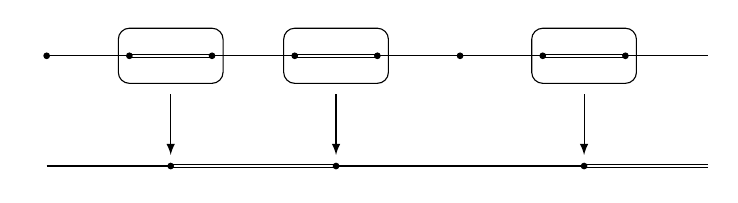
\begin{tikzpicture}[scale=.7]
    		\newcommand{\orig}{-1.5}
    		\newcommand{\trans}{1.5}
    		\newcommand{\vertspac}{-2.}
    		\newcommand{\vertsize}{.5} % vertical spand of the rectangles
    		\newcommand{\del}{.2}
    	
    		% initial chain
    	
    		% bonds 
        	\draw[-] (\orig, 0)  node [left] {}  -- (\orig+\trans, 0);
			\draw[-,double] (\orig+\trans,0) -- (\orig+2*\trans,0); % node [midway, above] {$t_s$};
			\draw[-] (\orig+2*\trans,0) -- (\orig+3*\trans,0); % node [midway, above] {$t_w$};	
			\draw[-,double] (\orig+3*\trans,0) -- (\orig+4*\trans,0); % node [midway, above] {$t_s$};
			\draw[-] (\orig+4*\trans,0) -- (\orig+5*\trans,0); % node [midway, above] {$t_w$};
			\draw[-] (\orig+5*\trans,0) -- (\orig+6*\trans,0); % node [midway, above] {$t_w$};
			\draw[-,double] (\orig+6*\trans,0) -- (\orig+7*\trans,0); % node [midway, above] {$t_s$};
			\draw[-] (\orig+7*\trans,0) -- (\orig+8*\trans,0); % node [midway, above] {$t_w$};
    	
    		% sites
			\foreach \x in {0,...,7}
		      \filldraw (\orig+\x*\trans,0) circle (0.05); % node [below] {$\ket{\x}$};
		      
		    % rectangles around molecules
		    \draw [rounded corners] (\orig +\trans-\del,-\vertsize) rectangle (\orig+2*\trans+\del,\vertsize);
		    \draw [rounded corners] (\orig +3*\trans-\del,-\vertsize) rectangle (\orig+4*\trans+\del,\vertsize);
		    \draw [rounded corners] (\orig +6*\trans-\del,-\vertsize) rectangle (\orig+7*\trans+\del,\vertsize);
		    
		    % arrows below rectangles
		    \draw [->] (\orig+1.5*\trans,-\vertsize-\del) -- (\orig+1.5*\trans,\vertspac+\del);
		    \draw [->] (\orig+3.5*\trans,-\vertsize-\del) -- (\orig+3.5*\trans,\vertspac+\del);
		    \draw [->] (\orig+6.5*\trans,-\vertsize-\del) -- (\orig+6.5*\trans,\vertspac+\del);
		      
			% molecular chains
			
			\foreach \x in {1}
			{
				\draw[-] (\orig, \x*\vertspac) node [left] {} -- (\orig+1.5*\trans, \x*\vertspac);
				\draw[-,double] (\orig+1.5*\trans, \x*\vertspac) -- (\orig+3.5*\trans, \x*\vertspac);
				\draw[-] (\orig+3.5*\trans, \x*\vertspac) -- (\orig+6.5*\trans, \x*\vertspac);
				\draw[-,double] (\orig+6.5*\trans, \x*\vertspac) -- (\orig+8*\trans, \x*\vertspac);
				
				\filldraw (\orig+1.5*\trans,\x*\vertspac) circle (0.05);
				\filldraw (\orig+3.5*\trans,\x*\vertspac) circle (0.05);
				\filldraw (\orig+6.5*\trans,\x*\vertspac) circle (0.05);
			}
		\end{tikzpicture}
		
		\item $ H_n = \left( z H_{n-2} - 1 \right) \oplus \left( \zb H_{n-3} \right) \oplus \left( z H_{n-2} + 1 \right) + \mathcal{O}(\rho^4) $
	\end{itemize}
    
\end{frame}

\begin{frame}{Fractal spectrum, fractal wavefunctions}
    {\centering
    	\includegraphics[scale=.9]{idos.pdf}
    	
     }
     
     {\centering
    	\includegraphics[scale=.5]{amplitude_wf.pdf}
    	
     }
\end{frame}

\begin{frame}{Multifractal analysis}

	\begin{columns}
	\begin{column}{5cm}
	\begin{itemize}
		\item $\alpha$ local zoom factor (scaling exponent)
		\item $f(\alpha)$ probability distribution of $\alpha$.
	\end{itemize}
	
     \end{column}
    
    \begin{column}{5cm}
    {\centering
    	\includegraphics[scale=.5]{f-alpha_04_to_06.pdf}
    	
     }
    \end{column}
   \end{columns}
\end{frame}

\end{document}
